%%%%%%%%%%%%%%%%%%%%%%%%%%%%%%%%%%%%%%%%%%%%%%%%%%%%%%%%%%%%%%%%%%%%%%%
% BAB 3
%%%%%%%%%%%%%%%%%%%%%%%%%%%%%%%%%%%%%%%%%%%%%%%%%%%%%%%%%%%%%%%%%%%%%%%

\mychapter{3}{BAB 3 TINJAUAN PUSTAKA}

% Donec vitae rutrum arcu. Aenean dictum mauris id lobortis
% vulputate. In ut pretium turpis. Nunc elit nunc, blandit et maximus
% at, maximus at orci. Aliquam a nisl pretium, eleifend odio sit amet,
% interdum augue. Donec magna elit, cursus gravida libero vitae, congue
% luctus sapien. Phasellus sit amet nisl sed nisl dictum
% porttitor. Etiam viverra lacus est, a ultrices nisi euismod ut.

\section{Aplikasi Web}
% \label{subsec:label}

Website merupakan kumpulan halaman Web yang saling berkaitan dan umumnya berada pada server yang sama serta memuat informasi yang disediakan oleh individu, kelompok, maupun organisasi. Website digunakan sebagai salah satu media untuk menyampaikan berbagai informasi kepada pengguna melalui jaringan Internet \parencite{Laksono2021}. Sejalan dengan pengertian tersebut, Kulakat, Utami, dan Wibowo menjelaskan bahwa website merupakan kumpulan dokumen daring yang berisi halaman Web dan terikat pada suatu domain sehingga dapat diakses oleh pengunjung melalui Internet. Informasi yang terdapat pada website dapat diakses oleh pengguna melalui halaman Web yang tersedia \parencite{Kulakat2021}.

Pada perkembangannya, website tidak hanya digunakan sebagai media penyampaian informasi yang bersifat statis, tetapi telah berkembang menjadi media yang lebih dinamis dan interaktif. Website dapat menyediakan berbagai fungsi sesuai dengan kebutuhan pengguna, seperti pengelolaan dan penyampaian data. Perkembangan tersebut didukung oleh penggunaan berbagai bahasa pemrograman dan teknologi pengembangan website, seperti HTML, PHP, CSS, JavaScript, serta basis data MySQL \parencite{Purbo2021}.

Pengembangan website dapat memanfaatkan framework untuk membantu proses pembangunan aplikasi. Framework menyediakan struktur dan fungsi yang dapat digunakan kembali sehingga pengembang tidak perlu membangun seluruh komponen aplikasi dari awal. Penggunaan framework juga dapat membantu pengembangan website menjadi lebih terstruktur dan mempermudah proses pengembangan serta pemeliharaan aplikasi \parencite{Purbo2021}.

% Dalam konteks pengembangan SIPANTAU, website digunakan sebagai media penyediaan layanan berbasis web yang memungkinkan pengguna dengan hak akses tertentu berinteraksi dengan aplikasi. Website tersebut digunakan untuk mendukung proses input data oleh dinas terkait serta menyediakan hasil prediksi kepada pengguna yang memiliki hak akses untuk melihat informasi tersebut.

\section{Backend}

Backend merupakan bagian aplikasi yang beroperasi pada sisi server dan bertanggung jawab terhadap interaksi dengan basis data serta logika fungsional program. Backend berkomunikasi dengan client melalui Application Programming Interface (API) \parencite{Nurhayati2023}. Dalam pengembangan aplikasi Web, backend merupakan bagian yang menangani proses pada sisi server. Jeng et al. menjelaskan bahwa pengembangan Web modern umumnya membagi tanggung jawab antara front-end dan back-end. Front-end bertanggung jawab terhadap tampilan halaman pada browser, termasuk gaya halaman, tata letak, pengalaman pengguna, dan fungsi aplikasi. Sementara itu, back-end bertanggung jawab terhadap akses data pada server, pengelolaan basis data, perancangan API, analisis, dan optimasi website \parencite{Jeng2021}.

Backend juga berperan dalam pengelolaan data yang digunakan oleh aplikasi. Proses tersebut dapat mencakup penyimpanan, pengambilan, pembaruan, dan penghapusan data pada basis data. Proses pengolahan data tersebut tidak dilakukan secara langsung oleh pengguna, tetapi diakses melalui antarmuka yang disediakan oleh backend untuk berkomunikasi dengan client \parencite{Nurhayati2023}. Komunikasi antara client dan backend dapat dilakukan melalui API. Client mengirimkan permintaan kepada backend, kemudian backend memproses permintaan tersebut sesuai dengan fungsi yang diperlukan dan memberikan respons kepada client. Pada pengembangan aplikasi Web, API menjadi salah satu komponen yang memungkinkan pemisahan tanggung jawab antara bagian antarmuka dan proses pada sisi server \parencite{Jeng2021,Nurhayati2023}.

\section{Model-View-Controller (MVC)}

Model-View-Controller (MVC) merupakan pola arsitektur yang memisahkan aplikasi menjadi tiga komponen utama, yaitu Model, View, dan Controller. Pemisahan tersebut bertujuan untuk memisahkan tanggung jawab antara data, antarmuka pengguna, dan proses aplikasi sehingga pengembangan dan pemeliharaan aplikasi dapat dilakukan secara lebih terstruktur
\parencite{Purbo2021}.

Model merupakan komponen yang berkaitan dengan logika bisnis dan pemrosesan data pada aplikasi. Model dapat melakukan akses terhadap sumber data, termasuk basis data, serta menangani proses yang berkaitan dengan data aplikasi. View bertanggung jawab terhadap logika tampilan dan proses rendering halaman yang ditampilkan kepada pengguna. Sementara itu, Controller berperan dalam mengatur alur aplikasi serta menangani berbagai event atau permintaan dari pengguna \parencite{Jeng2021}.

Alur kerja arsitektur MVC dimulai ketika pengguna mengirimkan request melalui browser kepada server. Server kemudian meneruskan request tersebut kepada Controller. Controller menentukan proses yang diperlukan dan berinteraksi dengan Model untuk membaca atau mengubah data. Data yang diperoleh dari Model kemudian diteruskan kepada View untuk menghasilkan tampilan halaman. Hasil rendering tersebut dikembalikan melalui Controller
dan server sebagai response kepada browser. Alur kerja arsitektur MVC tersebut ditunjukkan pada Gambar \ref{fig:mvc-architecture} \parencite{Jeng2021}.

\begin{figure}[H]
    \centering
    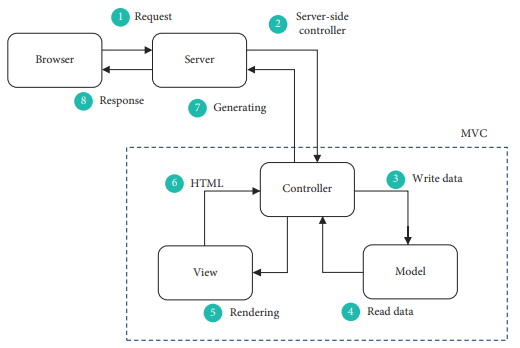
\includegraphics[width=\textwidth]{img/mvc-architecture.png}
    \caption{Arsitektur pengembangan Web menggunakan MVC}
    \label{fig:mvc-architecture}
    
    \vspace{-0.2cm}
    \begin{center}
        Sumber: Jeng et al. (2021)
    \end{center}
\end{figure}

Pola arsitektur MVC dapat diterapkan menggunakan berbagai bahasa pemrograman maupun framework dalam pengembangan aplikasi Web. Penerapan pola tersebut memungkinkan pengembang memisahkan pengelolaan data, tampilan, dan alur proses aplikasi berdasarkan tanggung jawab masing-masing komponen. Salah satu framework yang menerapkan pola MVC adalah Laravel, yaitu framework berbasis PHP yang menggunakan Model, View, dan Controller sebagai komponen utama dalam struktur aplikasinya \parencite{Purbo2021}. Dalam pengembangan SIPANTAU, Laravel digunakan sebagai framework pada sisi backend, dengan penerapan komponen Model dan Controller untuk mengelola data serta proses aplikasi. Komponen View tidak termasuk dalam lingkup pengembangan pada Praktik Kerja Lapang karena pengelolaan antarmuka pengguna dilakukan pada sisi frontend.

\section{Basis Data dan MySQL}

Basis data dan sistem manajemen basis data (\textit{Database Management System}/DBMS) merupakan dua komponen utama dalam sistem informasi. DBMS berkaitan dengan pengelolaan data yang terdapat dalam basis data dan menjadi salah satu komponen yang mendukung pengoperasian sistem informasi. Dalam pengelolaan basis data, \textit{Structured Query Language} (SQL) digunakan sebagai bahasa kueri untuk mengambil data dari basis data serta melakukan berbagai tugas pengelolaan data. SQL juga memiliki keterkaitan erat dengan DBMS karena sebagian besar DBMS modern menggunakan SQL sebagai bahasa kueri untuk mengelola data \parencite{Taipalus2021}. Dengan demikian, SQL menjadi salah satu bahasa yang digunakan dalam proses pengambilan dan pengelolaan data pada sistem manajemen basis data.

Salah satu model yang digunakan dalam pengelolaan basis data adalah model relasional. Pada model basis data relasional, data disusun dalam sekumpulan tabel yang dikelompokkan berdasarkan baris dan kolom. Tabel digunakan sebagai struktur untuk mengorganisasi data, sedangkan kolom merepresentasikan atribut dari data yang disimpan dan baris merepresentasikan entri atau rekaman data. Setiap rekaman dalam tabel dapat memiliki \textit{primary key} yang digunakan untuk mengidentifikasi rekaman secara unik. Selain itu, \textit{foreign key} dapat digunakan untuk menghubungkan tabel yang memiliki keterkaitan \parencite{Bonteanu2024}. Struktur tabel beserta hubungan antar-data tersebut digunakan untuk mengorganisasi informasi dalam basis data relasional.

MySQL merupakan salah satu sistem manajemen basis data relasional (\textit{Relational Database Management System}/RDBMS) yang bersifat \textit{open-source} dan memiliki basis pengguna yang luas. MySQL juga banyak digunakan dalam pengembangan aplikasi web serta menyediakan berbagai kemampuan untuk mendukung pengelolaan basis data, seperti replikasi, \textit{full-text search}, dan dukungan terhadap berbagai \textit{storage engine} \parencite{Bonteanu2024}. Dalam penerapannya sebagai basis data relasional, MySQL menyusun data dalam bentuk tabel yang memiliki kolom sebagai bagian dari struktur data \parencite{Gyrdi2021}. Győrödi et al. juga membedakan MySQL sebagai basis data relasional dengan \textit{document-based MySQL} sebagai pendekatan basis data non-relasional.

\section{Identification, Authentication, dan Role-Based Access Control Authorization}

Dalam sistem informasi, proses pengendalian akses terhadap sumber daya diawali dengan \textit{identification}, yaitu proses menghubungkan seseorang dengan identitas tertentu dari sejumlah identitas yang tersedia. Proses tersebut kemudian dilanjutkan dengan \textit{authentication} dan \textit{authorization}. \textit{Identification} berfungsi untuk menentukan identitas yang digunakan oleh pengguna dalam sistem dan \textit{Authentication} yang merupakan tahap berikutnya memastikan identitas yang diberikan memang milik orang tersebut \parencite{Bucko2023}.

\textit{Authentication} merupakan proses untuk menentukan apakah pengguna atau proses merupakan entitas yang sesuai dengan identitas yang diklaimnya. Proses ini memastikan bahwa entitas yang melakukan komunikasi dengan sistem merupakan entitas yang sah. Kredensial yang digunakan dalam \textit{authentication} dapat berupa sesuatu yang diketahui pengguna, seperti PIN atau kata sandi, sesuatu yang dimiliki pengguna, seperti kartu pintar atau sertifikat digital, serta karakteristik pengguna, seperti biometrik. Dengan demikian, \textit{authentication} berperan dalam memvalidasi pengguna sebelum sistem memberikan akses terhadap sumber daya yang dilindungi \parencite{Bucko2023}.

Setelah identitas pengguna berhasil diverifikasi melalui \textit{authentication}, sistem perlu menentukan hak akses yang dimiliki oleh pengguna tersebut. Proses ini disebut \textit{authorization}, yaitu teknik keamanan yang digunakan untuk menentukan privilege pengguna atau kesesuaiannya dalam melakukan tugas tertentu pada sistem. \textit{Authorization} merupakan tahapan setelah \textit{identification} dan \textit{authentication} dalam proses pemberian akses. Berbeda dengan \textit{authentication} yang menghasilkan keputusan mengenai keabsahan identitas, \textit{authorization} menentukan batasan akses pengguna terhadap berbagai sumber daya sistem sesuai dengan hak yang dimilikinya \parencite{Bucko2023}.

Salah satu strategi yang dapat digunakan dalam \textit{authorization} adalah \textit{Role-Based Access Control} (RBAC). Pada RBAC, hak akses tidak diberikan secara langsung kepada setiap pengguna, tetapi dikaitkan dengan role yang dimiliki pengguna. Role tersebut memiliki sekumpulan permission yang menentukan tindakan atau sumber daya yang dapat diakses. Kamboj et al. menjelaskan bahwa struktur RBAC terdiri atas tiga entitas utama, yaitu \textit{users}, \textit{roles}, dan \textit{permissions}, yang dihubungkan melalui hubungan \textit{user-role assignment} dan \textit{role-permission assignment}. Dengan pendekatan tersebut, permission dapat diberikan kepada pengguna berdasarkan role yang sesuai dengan tugas atau tanggung jawabnya \parencite{Kamboj2021}.

Penerapan access control tersebut juga relevan pada aplikasi berbasis web. Le et al. menjelaskan bahwa access control merupakan mekanisme keamanan untuk menentukan pengguna yang dapat mengakses suatu sumber daya serta tindakan yang dapat dilakukan terhadap sumber daya tersebut. Dalam aplikasi web, sumber daya dapat berupa halaman server, halaman client, gambar, maupun berkas lainnya, sedangkan permission dapat merepresentasikan kemampuan untuk mengakses suatu sumber daya melalui metode HTTP tertentu, seperti GET dan POST. Oleh karena itu, penerapan RBAC pada aplikasi web dapat digunakan untuk menentukan sumber daya dan operasi yang dapat dilakukan berdasarkan role pengguna \parencite{Le2022}.

\section{Integrasi Model Prediksi pada Aplikasi Berbasis Web}

Model machine learning yang telah dikembangkan dapat diintegrasikan ke dalam aplikasi berbasis web untuk menyediakan fungsi prediksi yang dapat digunakan secara langsung oleh pengguna. \cite{Alboaneen2022} misalnya, mengembangkan sistem prediksi berbasis web yang menggunakan model machine learning untuk memprediksi performa akademik mahasiswa. Sistem tersebut tersedia pada online server sehingga dapat digunakan oleh tutor. Hal ini menunjukkan bahwa aplikasi berbasis web dapat digunakan sebagai media untuk menyediakan hasil prediksi dari model machine learning kepada pengguna.

Dalam proses integrasi, model prediksi yang telah tersedia dapat digunakan sebagai komponen inference pada aplikasi tanpa harus melakukan pengembangan model dari awal. \cite{Goh2023} menjelaskan bahwa penggunaan kembali (reuse) model pre-trained merupakan salah satu pendekatan yang dapat digunakan dalam pengembangan aplikasi deep learning berbasis web. Pendekatan tersebut memungkinkan model yang telah dilatih sebelumnya untuk digunakan kembali dalam aplikasi sehingga proses pengembangan dapat difokuskan pada integrasi model dengan lingkungan aplikasi dan penyediaan antarmuka bagi pengguna.

Implementasi integrasi tersebut pada dasarnya melibatkan alur antara masukan pengguna, model prediksi, dan keluaran sistem. \cite{Mohammed2022} menunjukkan proses serupa ketika mengimplementasikan model prediksi yang sebelumnya dikembangkan dalam lingkungan R ke dalam aplikasi berbasis web. Setelah model dikonversi ke format yang kompatibel dengan JavaScript, pengguna dapat memasukkan data melalui halaman web, kemudian data tersebut diteruskan ke model untuk menghasilkan prediksi. Hasil prediksi selanjutnya dikembalikan dan ditampilkan pada halaman web.

Selain integrasi antara aplikasi dan model, kesesuaian format data juga menjadi bagian penting dalam proses inference. \cite{Mohammed2022} menunjukkan bahwa model yang dikembangkan menggunakan suatu lingkungan pemrograman belum tentu dapat langsung digunakan pada lingkungan aplikasi web sehingga diperlukan penyesuaian atau konversi agar model dapat dijalankan pada lingkungan target. Dalam penelitian tersebut, model yang dikembangkan menggunakan R dikonversi ke format yang kompatibel dengan JavaScript sebelum digunakan pada aplikasi web. Hal ini menunjukkan bahwa proses integrasi tidak hanya mencakup pemanggilan model, tetapi juga memastikan bahwa data masukan dan keluaran memiliki format yang sesuai dengan kebutuhan model dan aplikasi.

Pendekatan tersebut juga diterapkan pada EarthAIHub oleh \cite{Sit2023}, yang menyediakan platform berbasis web untuk menggunakan pre-trained deep learning models. Platform tersebut menggunakan abstraction layer untuk menjembatani aplikasi dengan model sehingga model dapat digunakan melalui platform yang sama. Konfigurasi model digunakan untuk mendefinisikan format masukan dan keluaran serta proses preprocessing dan postprocessing. Dengan demikian, integrasi model pada aplikasi dapat dipandang sebagai suatu alur yang mencakup penerimaan data masukan, penyesuaian data melalui preprocessing, proses inference menggunakan model, serta pengolahan keluaran sebelum ditampilkan kepada pengguna.

Berdasarkan pendekatan tersebut, integrasi model Chronos-v2 pada aplikasi SIPANTAU dilakukan dengan memanfaatkan model dan pipeline yang telah tersedia sebagai komponen prediksi. Aplikasi bertugas menyediakan antarmuka bagi pengguna untuk memasukkan data, meneruskan data tersebut ke komponen pipeline sesuai format yang dibutuhkan, menjalankan proses inference, serta mengolah hasil prediksi agar dapat ditampilkan kembali melalui antarmuka aplikasi. Dengan pendekatan ini, proses pengembangan SIPANTAU berfokus pada integrasi model yang telah tersedia ke dalam sistem aplikasi, bukan pada pembangunan dan pelatihan ulang model prediksi.

% \section{Dolor}
% \label{subsec:label}

% Curabitur vel tellus ligula. In consequat quam enim, sit amet
% ullamcorper est elementum nec. Vestibulum mattis congue
% tincidunt. Duis elementum erat ac varius rutrum. Proin sagittis, neque
% scelerisque sodales pharetra, nulla lacus ornare est, et cursus urna
% ex ut turpis. Morbi auctor, erat vitae semper cursus, nibh ipsum
% tristique lorem, maximus ultrices massa neque eu risus. Interdum et
% malesuada fames ac ante ipsum primis in faucibus.


% \section{Sit}
% \label{subsec:label}

% Curabitur vel tellus ligula. In consequat quam enim, sit amet
% ullamcorper est elementum nec. Vestibulum mattis congue
% tincidunt. Duis elementum erat ac varius rutrum. Proin sagittis, neque
% scelerisque sodales pharetra, nulla lacus ornare est, et cursus urna
% ex ut turpis. Morbi auctor, erat vitae semper cursus, nibh ipsum
% tristique lorem, maximus ultrices massa neque eu risus. Interdum et
% malesuada fames ac ante ipsum primis in faucibus.

% \begin{itemize}
% \item Dolor
% \item Sit
% \item Amet
% \end{itemize}


% \section{Penarikan Kesimpulan}
% \label{subsec:label}

% Phasellus porttitor purus \textcite{warn} vitae finibus laoreet. Class
% aptent taciti sociosqu ad litora torquent per conubia nostra, per
% inceptos himenaeos. Lorem ipsum dolor sit amet, consectetur adipiscing
% elit. Nunc tempus sed purus sit amet porta. Sed volutpat est ac arcu
% porttitor, non pharetra tortor pharetra. Phasellus vitae dictum
% elit. Curabitur elementum consequat elementum. Integer in vulputate
% metus. Aliquam erat volutpat. Phasellus vitae convallis orci. Etiam ac
% metus tristique, viverra metus a, mattis lectus. Aenean vel vestibulum
% augue.

% \section{Jadwal penelitian}
% \label{subsec:label}
